%\documentclass[journal]{new-aiaa}
\documentclass[conf]{new-aiaa}
\usepackage[utf8]{inputenc}
\usepackage{graphicx}
\usepackage{amsmath}
\usepackage{subcaption}
\usepackage{sidecap}
\usepackage{mathtools}
\usepackage{commath}
\usepackage{listings}
\usepackage[version=4]{mhchem}
\usepackage{siunitx}
\usepackage{algorithm}
\usepackage[linewidth=1pt]{mdframed}
\usepackage{algpseudocode}
\usepackage{longtable,tabularx}
\usepackage{amsmath,amsfonts,bm} % Math packages

\usepackage{amssymb}        % to get all AMS symbols
\usepackage{hyperref}       % PDF hyperreferences??
\usepackage[framed,numbered,autolinebreaks,useliterate]{mcode}

\renewcommand*\arraystretch{0.9}

\setlength\LTleft{0pt} 

\title{Optimal Guidance and Control Schemes for Spacecraft Rendezvous}

\author{Pádraig S. Lysandrou\footnote{PhD Student, Aerospace Engineering, AIAA Student Member}}
\affil{University of Colorado Boulder, Boulder, Colorado, 80301}
\affil{Final Project for ASEN6014: Spacecraft Formation Flying}


\begin{document}
\maketitle

\begin{singlespace}
\begin{abstract}
    \begin{itemize}
        In this final project for Spacecraft Formation Flying, we derive and employ optimal glideslope guidance and control technique for the rendezvous of two spacecraft where the target is an unpowered vehicle in a circular orbit. Many applications of spacecraft rendezvous require a constant straight-line approach such that the target vehicle can monitor the approaching one closely. This allows crew to act in the case of non-nominal conditions. The Clohessy-Wiltshire-Hill equations are posed in the radial-transversal frame and used to derive an optimal control solution for maintaining a constant glideslope approach. Then a PD control law is proposed for vehicles with off-slope initial conditions. The control usage is then compared to a nonlinear Lyapunov-based feedback control law.
    \end{itemize}
\end{abstract}

\section*{Nomenclature}
{\renewcommand\arraystretch{1.0}
\noindent\begin{longtable*}{@{}l @{\quad=\quad} l@{}}
$\mathbf{^Nr}_i$  	& Position vector, inertial frame\\
$\mathbf{^Nv}_i$  	& Velocity vector, inertial frame\\
$G$                  & Gravitational constant \\
$\bm{a}_x$          & Input acceleration on x axis \\
$n$               & Circular mean motion \\
$[x \ y \ z]$       & Position components, rectilinear frame \\
$J$             & Total Cost \\
$L[\cdot]$       & Cost Function Lagrangian \\
$\dot{m}$        & Mass flow rate \\
$I_{sp}$        & Specific Impulse \\
$\Phi$          & State Transition Matrix Function\\
$H$             & Hamiltonian Function \\
$\lambda$       & Costate Variable \\
$[r \ t]$       & Radial and Transversal Displacement Components \\
$\theta$        & Glideslope Approach Angle
\end{longtable*}}



\clearpage
\section{Introduction}
In this paper, we shall develop, implement, and test an optimal control law for spacecraft rendezvous on a glideslope line. By approaching the chief spacecraft on a glideslope, the crew on-board can observe the approaching spacecraft in the case of off-nominal conditions. Rendezvous requires the matching of position and velocity vectors in a safe manner such that the deputy spacecraft can slowly approach and dock or berth with the chief, unpowered spacecraft. Rendezvous occurs each time the International Space Station requires re-supplying or re-crewing. The Soyuz, ATV, and Dragon 2 employ autonomous docking to the ISS, where the Japanese HTV, Dragon 1, and Cygnus station-keep about one point and wait to be berthed via a robotic arm.

This report covers the following tasks as listed in the proposal:
\begin{itemize}
    \item Task 1: Implement the Zanetti Glideslope Guidance as per \cite{zanetti2011optimal}.
    \item Task 2: Implement a CWH proportional-derivative and Lyapunov controllers, then compare them
    \item Task 3: Look at the performance with the nonlinear dynamics, uncertain initial conditions, and noise in the control
\end{itemize}
All tasks are completed and documented in the following sections.
%
\section{Task 1: Zanetti Guidance Implementation}
We shall describe the Hill frame coordinate system, which is the predominant frame in use. The position of the deputy vehicle (the vehicle making maneuvers) is the following:
\begin{equation}\label{relativedefinition}
    \bm{r}_d = \bm{r}_c + \bm{\rho} = (r_c + x)\bm{\hat{o}}_r + y\bm{\hat{o}}_\theta + z \bm{\hat{o}}_h
\end{equation}
The DCM transforming an inertial frame vector to a Hill frame one is described as such: $[HN] = [\bm{\hat{o}}_r^T \ \bm{\hat{o}}_\theta^T \ \bm{\hat{o}}_h^T]^T$. Instantaneously each vector can be found with $\bm{\hat{o}} = \frac{\bm{r}}{\norm{\bm{r}}}$, $\bm{\hat{o}}_h = \frac{\bm{r}\times\bm{v}}{\norm{\bm{r}\times\bm{v}}}$, and $\bm{\hat{o}}_\theta = \bm{\hat{o}}_h \times \bm{\hat{o}}_r$ \cite{sj}.

First, let us assume the linear Clohessy Wiltshire equations of motion, which describe the relative motion of the two spacecraft:
\begin{align}
    \ddot{x} - 2n\dot{y} -3n^2x &= 0 \\
    \ddot{y} + 2n\dot{x} &= 0 \\
    \ddot{z} + n^2z &=0 
\end{align}
Solving and including input accelerations, we have the following:
\begin{align}
    \ddot{x} &= 2n\dot{y} + 3n^2x + u_x \\
    \ddot{y} &= - 2n\dot{x} + u_y \\
    \ddot{z} &= - n^2z + u_z 
\end{align}
For simplicity, we may also call our Hill frame: $\{\bm{\hat{o}}_r \ \bm{\hat{o}}_\theta \ \bm{\hat{o}}_h\} = \{\bm{\hat{x}} \ \bm{\hat{y}} \ \bm{\hat{z}}\}$. This formulation differs from Zanetti in that we have that $\bm{\hat{x}}= \bm{\hat{y}}_{Zanetti}$ and $\bm{\hat{y}}= -\bm{\hat{x}}_{Zanetti}$.

For a continuously thrusting propulsion system, an appropriate performance criteria is the quantity of propellant use. We use a Lagrange type cost function to describe the performance:
\begin{align}
    \mathcal{J} = \int_0^{t_f} L[\cdot] \  dt = \frac{1}{2}\int_0^{t_f} \mathbf{u}^T \mathbf{u} dt
\end{align}

This cost function will be subject to our linear CWH dynamics and the continuous glideslope constraint for constant direction rendezvous approaches. Generally, propulsive thrusters follow the following mass flow rate relation:
\begin{align}
    \dot{m}= \frac{T}{I_{sp}g_0} 
\end{align}
Electric thrusters follow the specific impulse law:
\begin{align}
    I_{sp} = \frac{2P}{g_0T}
\end{align}

Let us defined the glideslope as a cone revolved around the negative x axis (or negative $\bm{\hat{o}}_r$) with angle $\theta$ off this axis. The glideslope defines a region between the approach direction and the negative x axis. The direction along the line of approach is called the radial direction $r$ and the in-plane perpendicular is called the transversal $t$. We perform a simple rotation to get these components:

\begin{align}
    \begin{bmatrix}
    r \\ t
    \end{bmatrix}
    &=
    \begin{bmatrix}
    \sin{\theta} & -\cos{\theta} \\
    \cos{\theta} & \sin{\theta} 
    \end{bmatrix}
    \begin{bmatrix}
    x \\ y
    \end{bmatrix} \\
    \bm{h} &= [R] \bm{c}
\end{align}
and therefore, we know that $\bm{c} = [R]^T\bm{h}$ where $ \text{det} ([R]) = +1 $ being in the SO(2) group family. We can also apply this rotation to the other state time derivatives $\dot{\bm{c}}$ and $\ddot{\bm{c}}$ similarly. After substitution, we then have the following dynamics:
\begin{align}
    \ddot{r} &= -3rn^2{\cos\left({\theta}\right)}^2+3t\sin\left({\theta}\right)n^2\cos\left({\theta}\right)+3rn^2+2{\dot{t}}n-{u_y}\cos\left({\theta}\right)+{u_x}\sin\left({\theta}\right) \\
    \ddot{t} &= 3tn^2{\cos\left({\theta}\right)}^2+3r\sin\left({\theta}\right)n^2\cos\left({\theta}\right)-2{rd}n+{u_x}\cos\left({\theta}\right)+{u_y}\sin\left({\theta}\right) \\
    \ddot{z} &= - n^2z + u_z 
\end{align}
We can of course take the same transformation to find $u_r$ and $u_t$ components:
\begin{align}
    \begin{bmatrix}
    u_r \\ u_t
    \end{bmatrix}
    &=
    \begin{bmatrix}
    \sin{\theta} & -\cos{\theta} \\
    \cos{\theta} & \sin{\theta} 
    \end{bmatrix}
    \begin{bmatrix}
    u_x \\ u_y
    \end{bmatrix}   
\end{align}
After this simple substitution, we arrive at the following:
\begin{align}
    \ddot{r} &= 2n{\dot{t}}+3n^2r\sin^2\theta+3n^2t\sin\theta\cos\theta + u_r\\
    \ddot{t} &= -2n\dot{r} +3n^2r\sin\theta\cos\theta + 3n^2t\cos^2\theta + u_t \\
    \ddot{z} &= - n^2z + u_z 
\end{align}
The problem at hand requires approaching the vehicle in a straight line, meaning that the transversal components must remain zero $t=\dot{t}=\ddot{t}=0$. Once applied to the dynamics above, we have that
\begin{align}
    \ddot{r} &= 3n^2 r \sin^2\theta + u_r\\
    0 &= -2n\dot{r} +3n^2r \sin\theta\cos\theta + u_t \\
    \ddot{z} &= - n^2z + u_z 
\end{align}
Solving for the transverse acceleration, we have that is must be $u_t^\star = 2n\dot{r} - 3n^2r\sin(\theta)\cos(\theta)$. Because the desired approach direction is within the plane of motion of the target vehicle, most methods seek to null out the out-of-plane components of motion very early on in the rendezvous phase. We can substitute this into our quadratic cost function.
\begin{align}
    \mathcal{J} = \frac{1}{2}\int_0^{t_f} u_r^2 + u_t^2 dt = \frac{1}{2}\int_0^{t_f} u_r^2 + (2n\dot{r} - 3n^2r\sin\theta\cos\theta)^2dt
\end{align}

This cost function is subject to the kinematic constraints $\dot{r} = v$ and $\dot{v}= 3n^2 r \sin^2\theta + u_r $. They are also subject to our initial and terminal boundary constraints:
\begin{align}
    r(0) = r_0 \quad v(0) = v_0 \quad r(t_f) = r_N \quad v(t_f) = v_N
\end{align}
Therefore, the Hamiltonian of the system is then the following:
\begin{align}
    H &= L[\cdot] + \boldsymbol{\lambda}^T \bm{f}[\cdot] \\
      &=\frac{1}{2} [u_r^2 + (2n\dot{r} - 3n^2r\sin\theta\cos\theta)^2]+ \lambda_rv + \lambda_v(3n^2 r \sin^2\theta + u_r)
\end{align}
We can find the costate dynamical equations $\dot{\lambda}_r, \ \dot{\lambda}_v$ via the partials:
\begin{align}
    \dot{\lambda}_r &= -\frac{\partial H}{\partial r} = 
        3n^3\cos{\theta}\sin{\theta}\left(2\dot{r}-3nr\cos{\theta}\sin{\theta}\right) - 3n^2\sin^2\theta \lambda_v \\
    \dot{\lambda}_v &= -\frac{\partial H}{\partial v} =  -\frac{\partial H}{\partial \dot{r}} =  2n^2(3nr\sin\theta \cos\theta -2\dot{r}) - \lambda_r
\end{align}
The control optimality condition, coming from the stationarity condition, is evaluated to be
\begin{align}
    \frac{\partial H}{\partial u_r} = u_r + \lambda_v = 0
\end{align}

Therefore the optimal control is clearly the negative of the velocity costate: $u_r = -\lambda_v$. Let us now augment the state vector to include the costate dynamics.
\begin{align}
    \frac{d}{dt}
    \begin{bmatrix}
        r \\ v \\ \lambda_r \\ \lambda_v
    \end{bmatrix}
    = \frac{d}{dt} \bm{x} = A\bm{x}
\end{align}
The $A$ matrix is the new dynamics matrix defined by:
\begin{align}
    A = 
    \begin{bmatrix}
        0 & 1 & 0 & 0 \\
        3n^2sin^2\theta & 0 & 0 & -1 \\
        -9n^4\cos^2\theta\sin^2\theta & 6n^3\cos\theta\sin\theta & 0 & - 3n^2\sin^2\theta \\
        6n^3\sin\theta \cos\theta & -4n^2 & -1 & 0
    \end{bmatrix}
\end{align}

We can then write the state transition matrix for this augmented system, and separate into a block form for each $\in \mathbb{R}^{2\times 2}$.
\begin{align}
    \Phi(\tau,t_0) = e^{A(\tau-t_0)} =
    \begin{bmatrix}
        \Phi_{rr}(\tau,t_0) & \Phi_{r\lambda}(\tau,t_0) \\
        \Phi_{\lambda r}(\tau,t_0) & \Phi_{\lambda\lambda}(\tau,t_0) \\
    \end{bmatrix}
\end{align}

Now let us use the STM in block form to find the initial conditions of the costate vector:

\begin{align}
    \begin{bmatrix}
        r_f \\ v_f \\ \lambda_{r_f} \\ \lambda_{v_f}
    \end{bmatrix}
    & =
    \Phi(t_f,t_0)
    \begin{bmatrix}
        r_0 \\ v_0 \\ \lambda_{r_0} \\ \lambda_{v_0}
    \end{bmatrix} \\
    & =
    \begin{bmatrix}
        \Phi_{rr}(t_f,t_0) & \Phi_{r\lambda}(t_f,t_0) \\
        \Phi_{\lambda r}(t_f,t_0) & \Phi_{\lambda\lambda}(t_f,t_0) \\
    \end{bmatrix}
    \begin{bmatrix}
        r_0 \\ v_0 \\ \lambda_{r_0} \\ \lambda_{v_0}
    \end{bmatrix}
\end{align}

Given that our terminal state is known and constrained, we can simplify the calculation using the block form to the following:
\begin{align}
    \begin{bmatrix}
        r_f \\ v_f
    \end{bmatrix}
    &= \Phi_{rr}(t_f,t_0)
    \begin{bmatrix}
        r_0 \\ v_0
    \end{bmatrix}
    +
    \Phi_{r\lambda}(t_f,t_0)
    \begin{bmatrix}
        \lambda_{r_0} \\ \lambda_{v_0}
    \end{bmatrix}
\end{align}
%
Solving for the costate we get this simple equation for the initial condition vector:
\begin{align}
    \begin{bmatrix}
        \lambda_{r_0} \\ \lambda_{v_0}
    \end{bmatrix}
    = \Phi_{r\lambda}(t_f,t_0)^{-1}
    \left(
    \begin{bmatrix}
        r_f\\v_f
    \end{bmatrix}
    -
    \Phi_{rr}(t_f,t_0)
    \begin{bmatrix}
        r_0\\v_0
    \end{bmatrix}\right)
\end{align}
Now that we know the entire initial condition vector, we can form the optimal control law at each point in time $u_r^\star(t) = -\lambda_v(t) \quad \forall t \in [t_0, t_f]$ as the following:
% \begin{mdframed}
    \begin{align}
        u_r^\star(t) = [0 \ \ 0 \ \ 0 \ -1]\Phi(t,t_0)\bm{x}_0
    \end{align}
% \end{mdframed}
Or, in a discrete form, we can simplify this for computation such that we only have to keep the costate from the last step.
\begin{align}
    u_r^\star[k+1] = [0 \ \ 0 \ \ 0 \ -1]\Phi(dt,0)\bm{x}[k]
\end{align}
Therefore the state transition matrix does not need to be evaluated at every step. We can use a single discrete step STM and keep track of the state and costate values. We simply just use the previous state and transition it by one step. We can select the input, or negative $\lambda_v$ costate, with a simple inner product.

The optimal control should satisfy the cost function with the following inequality:
\begin{align}
    \mathcal{J}^\star \triangleq \frac{1}{2}\int_0^{t_f} {\bm{u}^\star}^T \bm{u}^\star dt \leq  \frac{1}{2}\int_0^{t_f} {\bm{u}}^T \bm{u} dt
\end{align}
One can employ the Weierstrauss and Legendre-Clebsh conditions to show that this solution is in fact minimum. The Weierstrauss condition requires that the Hamiltonian at an admissible control $u_r$ shall have cost greater or equal to that of the Hamiltonian evaluated at the optimal control $u_r^\star$. Therefore
\begin{align}
    H(u_r) - H(u_r^\star)= \frac{1}{2}(u_r^2 - {u_r^\star}^2) + \lambda_v(u_r -  {u_r^\star}^2) \geq 0
\end{align}
Knowing that $ u_r^\star = -\lambda_v $, we substitute to get this inequality:
\begin{align}
    H(u_r) - H(u_r^\star)= \frac{1}{2}(u_r - {u_r^\star})^2 \geq 0
\end{align}
The second order partial of the Hamiltonian with respect to the optimal control should be positive definite, according to the Legendre-Clebsh condition of optimality. It is easy to see that
\begin{align}
    \frac{\partial^2 H}{\partial u_r^2} = 1
\end{align}
which satisfies this condition; the proposed optimal control decision is a minimum.


\subsection{V-bar Approach Example}
Now let us look at an example where the deputy is approaching the chief in the $+\bm{\hat{o}}_\theta$ or ``from the front''. This means that the glideslope approach angle is $\theta = \pi$. The deputy is 200 meters in front of the chief vehicle at the same velocity. Figure \ref{fig:traj_v} shows the vehicle approaching directly on the glideslope to the chief. The terminal Hill velocity constraint is met at the final time of $\frac{1}{5}$ of an orbit at 400km as seen in \ref{fig:vels_v}. The control history for this scenario is shown in figure \ref{fig:v2}. These are results of a non-linear simulation of the 2-body dynamics, with control determined by the optimal policy.

The implementation of this optimal control law \textbf{completes Task 1}.

 \begin{figure}[htpb!]
\begin{subfigure}{.5\textwidth}
  \centering
  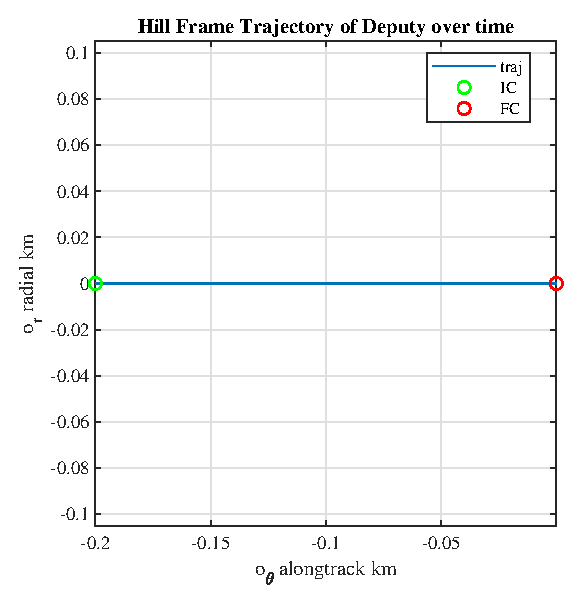
\includegraphics[width=.8\linewidth]{figures/traj.eps}
  \caption{Deputy trajectory in the Hill Frame, $\rho_0 = [0  \ 0.2 \ 0], \theta=\pi $}
  \label{fig:traj_v}
\end{subfigure}%
\begin{subfigure}{.5\textwidth}
  \centering
  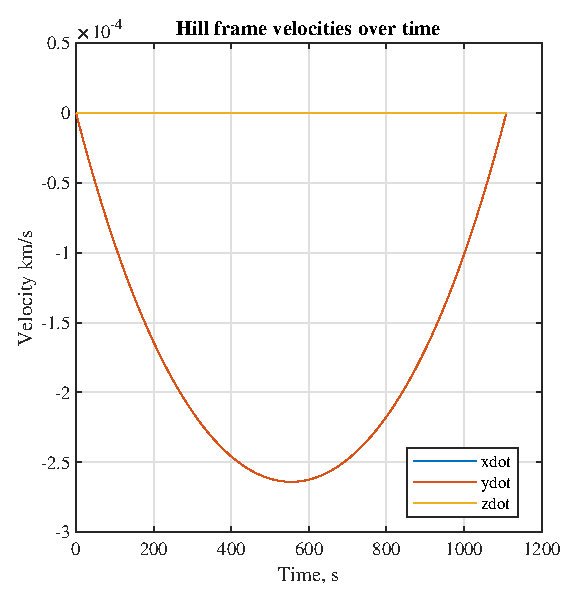
\includegraphics[width=.8\linewidth]{figures/hillvels.eps}
  \caption{Deputy Velocities in the Hill Frame}
  \label{fig:vels_v}
\end{subfigure}
\caption{V-Bar approach, front-approaching deputy ($+\bm{\hat{o}}_\theta$)}
\label{fig:v1}
\end{figure}

\begin{figure}[!htbp] 
  \centering
  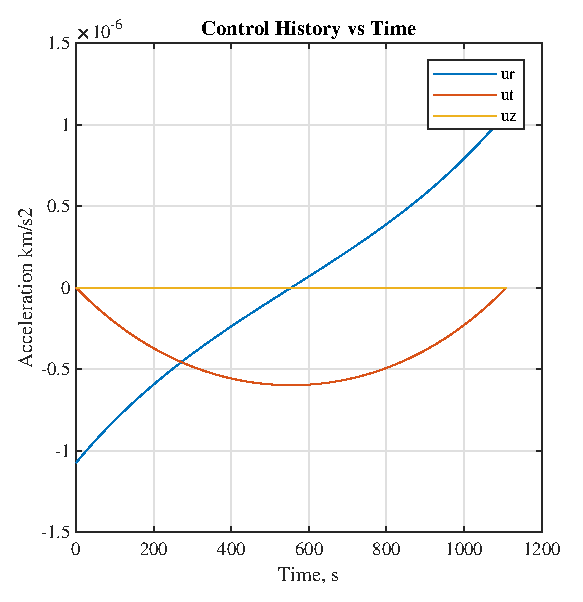
\includegraphics[width=0.5\textwidth]{figures/controls.eps}
  \caption{Radial-Transverse Frame Control History}
  \label{fig:v2}
 \end{figure}


\clearpage
\section{Task 2: Zanetti PD Comparison with Lyapunov Controller}
The optimal input control for the radial and transverse directions assume that the vehicle is on the glideslope and that $t = \dot{t} = \ddot{t} = 0$. However, it is not pragmatic to assume that initial state will be well conditioned. The law proposed by Zanetti is the following:
%
\begin{align}
    u_r &= u_r^\star - 2n\dot{t} - 3n^2t\sin\theta\cos\theta \\
    u_t &= u_t^\star - 3n^2t\cos^2\theta - k_pt -k_d\dot{t} \\
    u_z &= -k_z\dot{z}
\end{align}
%
\subsection{R-bar Approach Example}
Now let us look at the R-bar approach where the deputy moves to the chief from below, or moves in the positive $\bm{\hat{o}}_r$ direction with a negative initial condition. Replicating the Zanetti text, the initial position of the deputy is 200 meters below the chief and slightly offset by 10 meters in the $+\bm{\hat{o}}_\theta$ direction. This means that the initial condition is off the glideslope and therefore the optimal control will not suffice. A proportional-derivative controller is combined with the optimal glideslope control to cancel these errors. These are results of a \textit{linear simulation of the CWH equations}, with control determined by the optimal policy.
%
%
\begin{figure}[htpb!]
\begin{subfigure}{.5\textwidth}
  \centering
  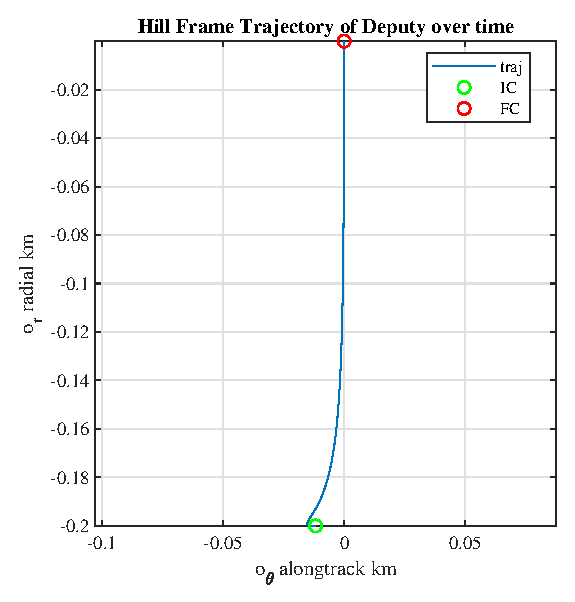
\includegraphics[width=.8\linewidth]{figures/traj_R.eps}
  \caption{Deputy trajectory in the Hill Frame, $\rho_0 = [-0.2  \ 0.01 \ 0], \theta=\frac{-\pi}{2} $}
  \label{fig:traj_r}
\end{subfigure}%
\begin{subfigure}{.5\textwidth}
  \centering
  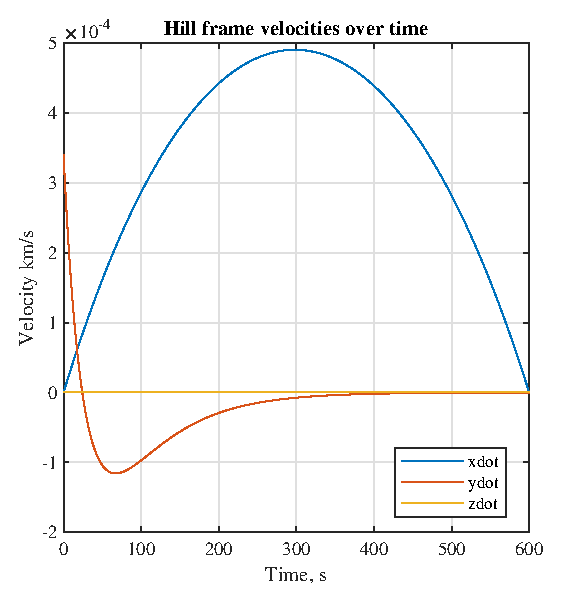
\includegraphics[width=.8\linewidth]{figures/hillvels_R.eps}
  \caption{Deputy Velocities in the Hill Frame}
  \label{fig:vels_r}
\end{subfigure}
\caption{Optimal Control Solution   R-Bar approach from ($-\bm{\hat{o}}_r$)}
\label{fig:v1}
\end{figure}

Figure \ref{fig:traj_r} shows the vehicle converging onto the glide slope and docking with the chief at zero velocity. The velocities and controls also converge quickly in figure \ref{fig:vels_r} and \ref{fig:comps}. The deputy vehicle provides initial significant thrust to start moving towards the chief, then a relatively constant rate-of-change braking thrust to slow down to zero velocity at the final state. Keep in mind that the gains must be tuned properly such that there is no overshoot. Nothing in this optimal control law is held to make sure that a collision, perhaps caused by controller overshoot, does not happen. It should be known that the gains used in this example were $K_p = .0005$, $K_d =0.05$, and $K_z = 0.003$. 
We shall use this as a prototype example for comparing this controller to a Lyapunov controller. 



\clearpage
\subsection{Lyapunov Based Cartesian Controller}
We now shall compare the same situation with a Lyapunov-derived globally stabilizing controller, derived in class, given by:
\begin{align}
    ^\mathcal{N}\boldsymbol{u}=-\left(\boldsymbol{f}\left(\boldsymbol{r}_{d}\right)-\boldsymbol{f}\left(\boldsymbol{r}_{d_{d}}\right)\right)-\left[K_{1}\right] \Delta \boldsymbol{r}-\left[K_{2}\right] \Delta \boldsymbol{\dot { r }}
\end{align}
The $\boldsymbol{f}\left(\boldsymbol{r}_{d}\right)$ term denotes the natural two-body acceleration from the deputy, and $\boldsymbol{f}\left(\boldsymbol{r}_{d_{d}}\right)$ denotes the two-body acceleration from the desired position. The $\Delta\bm{r}$ term is equal to $\bm{r}_d - \bm{r}_{d_d}$ and $\Delta\dot{\bm{r}} = \dot{\bm{r}_d} - \dot{\bm{r}}_{d_d}$. Of course the desired position and velocities in this case are that of the chief.

For the very same R-bar case as seen above, we now \textit{simulate the nonlinear dynamics} with this controller. We see that in figure \ref{fig:trajLyap}, the deputy does not approach the chief from the desired glideslope direction.
\begin{figure}[htpb!]
\begin{subfigure}{.5\textwidth}
  \centering
  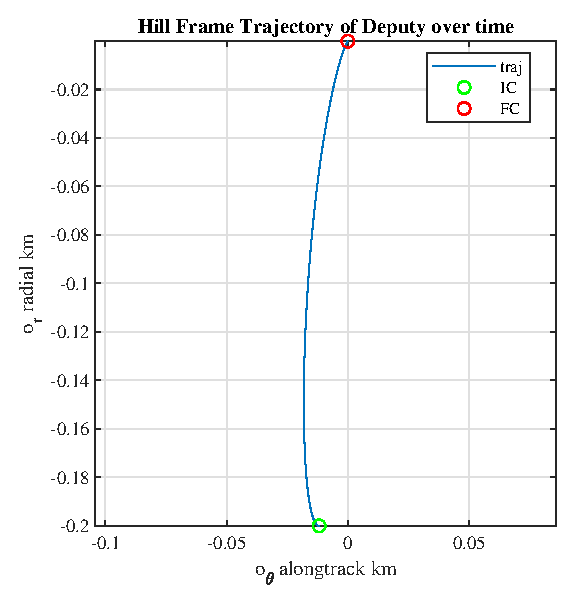
\includegraphics[width=.8\linewidth]{figures/trajLyap.eps}
  \caption{Deputy trajectory in the Hill Frame}
  \label{fig:trajLyap}
\end{subfigure}%
\begin{subfigure}{.5\textwidth}
  \centering
  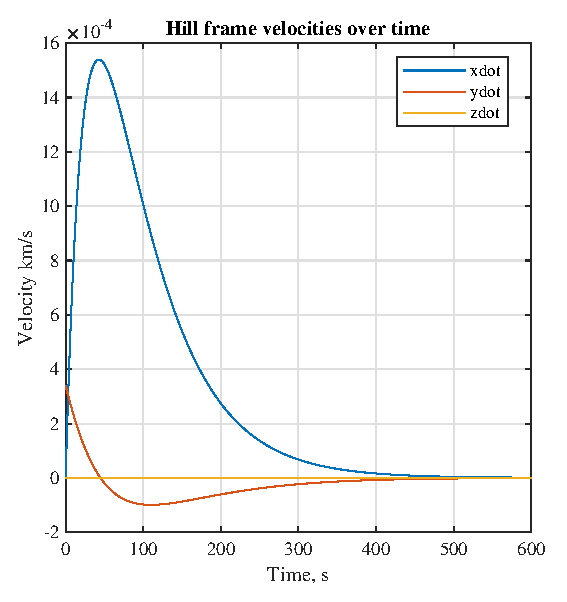
\includegraphics[width=.8\linewidth]{figures/velsLyap.eps}
  \caption{Deputy Velocities in the Hill Frame}
  \label{fig:velsLyap_r}
\end{subfigure}
\caption{R-Bar Approach Using Lyapunov PD Control Law}
\label{fig:v1}
\end{figure}




\subsection{A Comparison of The Optimal and Lyapunov Laws}
Obviously, we should not expect the Lyapunov based controller to meet any of the glideslope guarantees necessarily. Obviously the optimal control derived  uses the essential assumption that we regulate to this glideslope. Therefore, one would not use a generic controller to constrain motion like this. Figure \ref{fig:comps} shows that the Lyapunov controller converges more quickly in velocity for the same PD gains. However, the simulation and optimal control were engineered such that they both converged in the same time to our desired position and velocity with some tolerance. Therefore, we can then compare their performance. Additionally, both cases used control in the \textit{two-body nonlinear dynamics simulation environment}.

The optimal control history over time shows the vehicle regulating immediately to the glideslope and then slowly braking it's way up to the chief target point in a straight line. Additionally, as expected, we see that the optimal control law has nearly half the $dV$ cost of the general Lyapunov controller. The optimal control minimizes the control cost, where the Lyapunov approach is myopic to control usage.

Figure \ref{fig:tvc} shows the Hill frame control vector over time plotted on the Hill frame trajectory. It becomes more apparent that the initial input magnitude is  high, forcing the vehicle to the glideslope. Then, as the vehicle approaches the chief, it performs retrograde braking burns in order to hit the terminal state with zero velocity. There is no overshoot.

This comparison \textbf{completes Task 2}.



\begin{figure}[htpb!]
\begin{subfigure}{.5\textwidth}
  \centering
  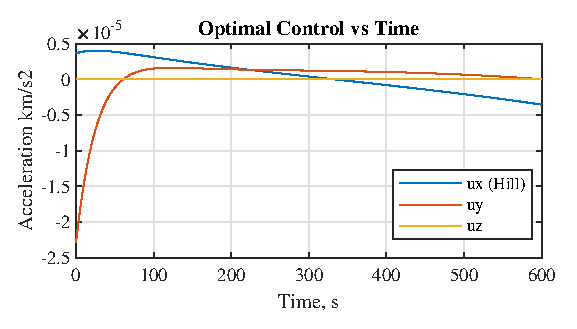
\includegraphics[width=.8\linewidth]{figures/controlsH.eps}
\end{subfigure}%
\begin{subfigure}{.5\textwidth}
  \centering
  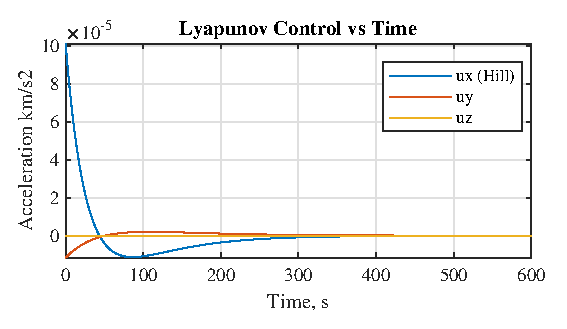
\includegraphics[width=.8\linewidth]{figures/controlsCart.eps}
\end{subfigure}
\\
\begin{subfigure}{.5\textwidth}
  \centering
  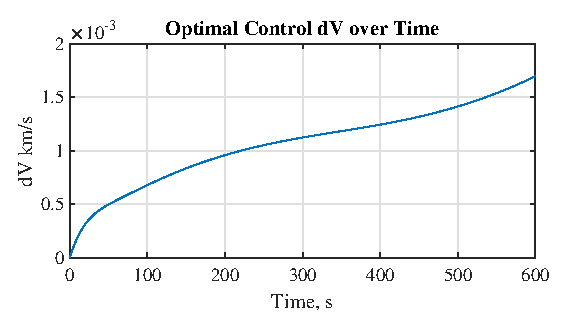
\includegraphics[width=.8\linewidth]{figures/dVOptimal.eps}
\end{subfigure}%
\begin{subfigure}{.5\textwidth}
  \centering
  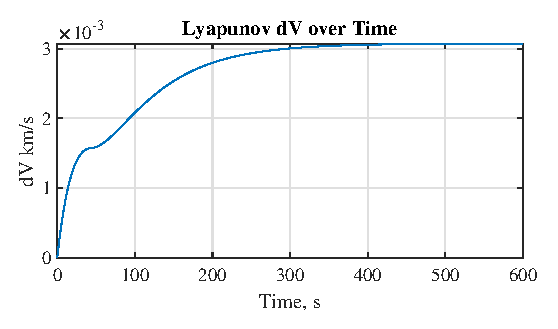
\includegraphics[width=.8\linewidth]{figures/dVCart.eps}
\end{subfigure}
\caption{$\Delta V$ Cost and Control History Comparison, R-Bar Approach Maneuver, Nonlinear Simulation}
\label{fig:comps}
\end{figure}

\begin{figure}[!htbp] 
  \centering
  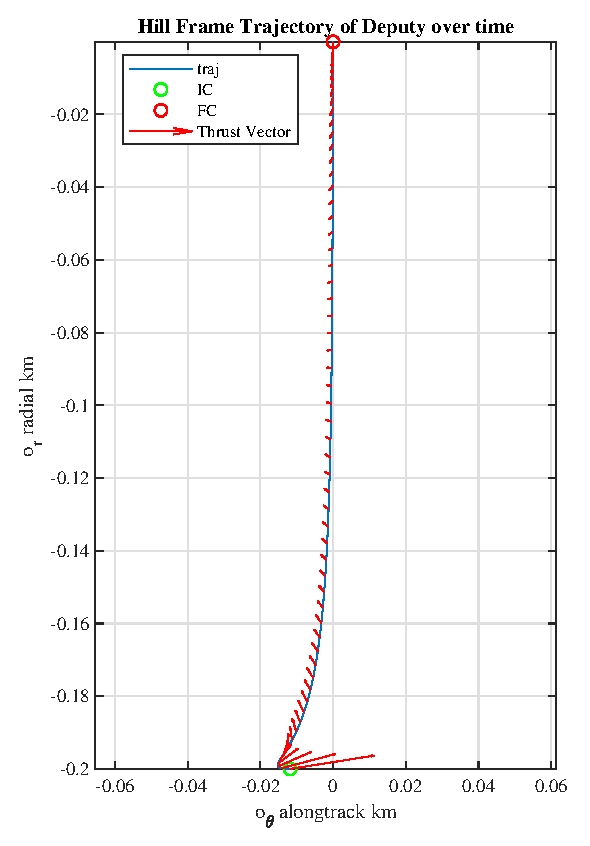
\includegraphics[width=0.5\textwidth]{figures/traj_quiv.eps}
  \caption{Optimal Control R-Bar Approach with Thrust Vector Quivers}
  \label{fig:tvc}
 \end{figure}



\clearpage
\section{Task 3: Testing Under Differing Conditions and Accuracy Comparison}

\subsection{Nonlinear Simulation Accuracy}
Simulating a scenario where the initial orbital conditions of the same as that shown in the R-bar approach shown in figure \ref{fig:tvc}, we see that the system behaves a little differently. The control history shown in \ref{fig:compsnl} and velocities in \ref{fig:offset} change towards to end of the trajectory to continue regulating. The terminal state of this simulation is offset from target by 0.4 meters in Hill frame displacement and 4 centimeters per second in Hill frame velocity in figure \ref{fig:offset}. While this may not seem a lot, we must consider the error that may build up over longer final times, different initial conditions and other factors. The $\Delta V$ cost difference, in this scenario, is negligible.
\begin{figure}[htpb!]
\begin{subfigure}{.5\textwidth}
  \centering
  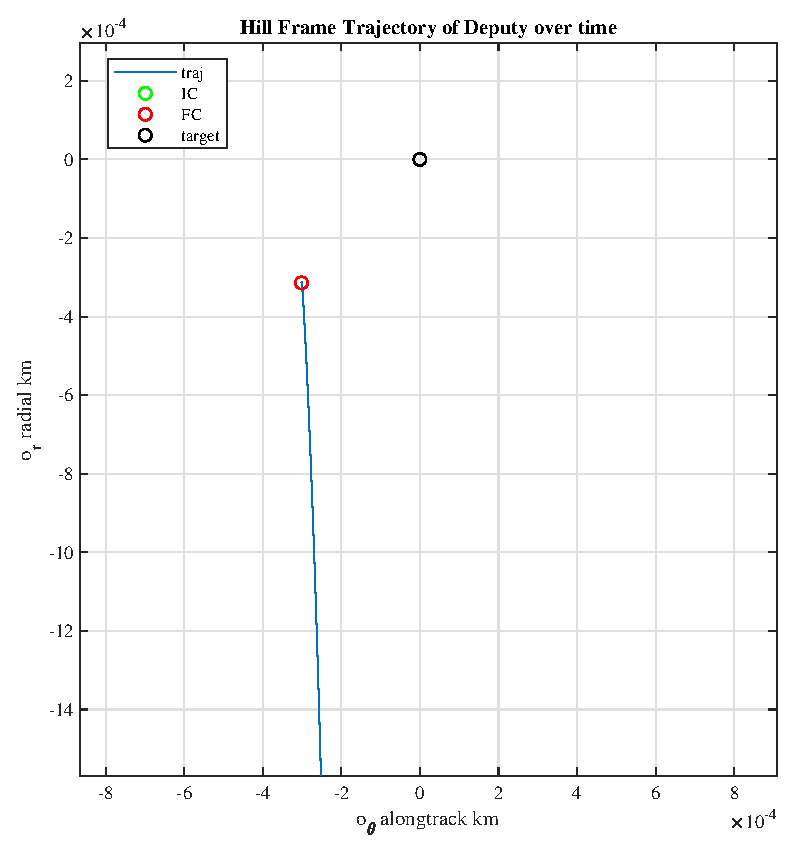
\includegraphics[width=0.8\textwidth]{figures/nlt3.eps}
  \caption{In-plane Motion Showing Offset Terminal State}
  \label{fig:offset}
\end{subfigure}%
\begin{subfigure}{.5\textwidth}
  \centering
  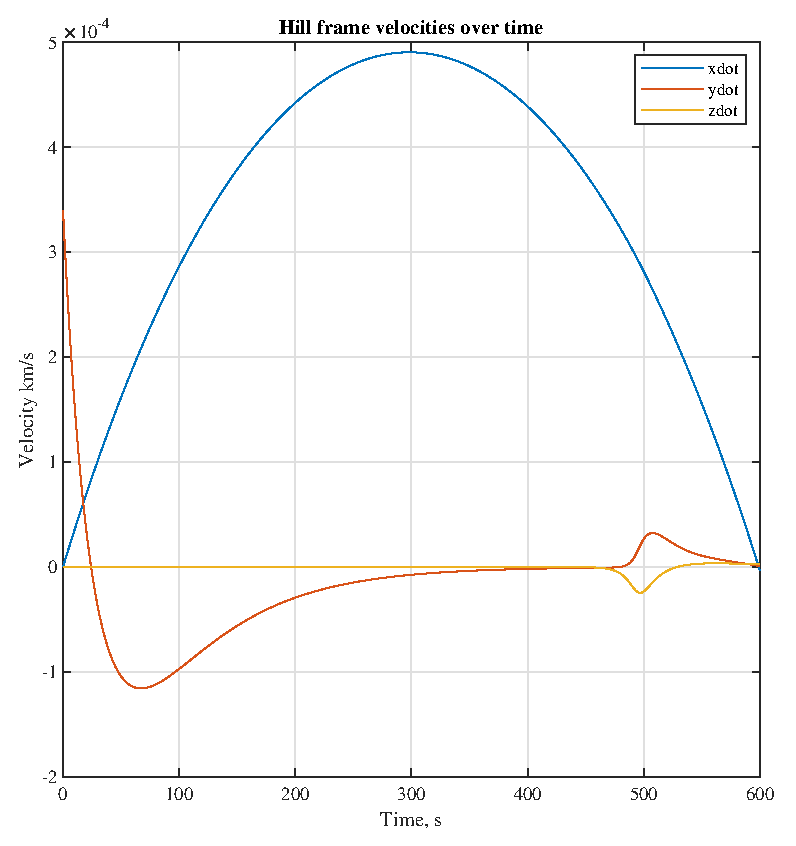
\includegraphics[width=0.8\textwidth]{figures/vels_N.eps}
  \caption{Hill Frame Velocities}
  \label{fig:offset}
\end{subfigure}
\label{fig:offsets}
\caption{Optimal Control in Nonlinear Simulation}
\end{figure}
\begin{figure}[htpb!]
\begin{subfigure}{.5\textwidth}
  \centering
  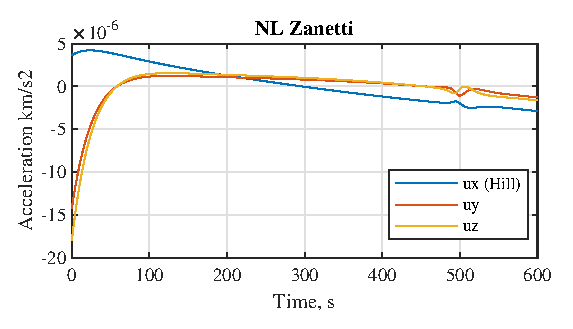
\includegraphics[width=.8\linewidth]{figures/controls_NL.eps}
\end{subfigure}%
\begin{subfigure}{.5\textwidth}
  \centering
  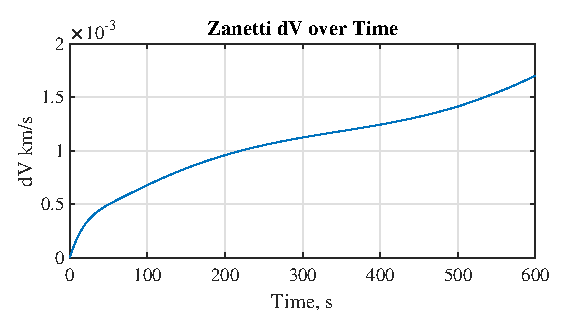
\includegraphics[width=.8\linewidth]{figures/dV_NL.eps}
\end{subfigure}
\caption{Control History and $\Delta V$ Consumption in Nonlinear Simulation}
\label{fig:compsnl}
\end{figure}




\subsection{Final Time and Accuracy Analysis}
As we vary the final time of the STM that is used to determine the optimal control history, the accuracy of the terminal state changes. For an R-bar approach case where we have $\delta a = -0.2$ and $\delta M_0 = .0001$, we see that there tends to be a nominal time-to-complete. With this optimal and PD control implementation, and this problem setup, some maneuvers are completed with higher accuracy in shorter periods of time. This means that the optimal control problem should be designed such that the time for completion is optimal as well, make it a free-final-time problem. As proposed currently, it is a fixed-final-time solution. Figure \ref{fig:finaltime} shows how the Hill frame position and velocity errors grow as the final time of the solution is extended. The plot shows error in meters and meters per second. It should also be known that the gains of the PD controller may want to redesigned for these cases, whereas the plot shown retains the same gain for each simulation run.

The relationship shown in \ref{fig:finaltime} means that an outer time of flight linear program can be written to find the right value for the solution. 
%
\begin{figure}[!htbp] 
  \centering
  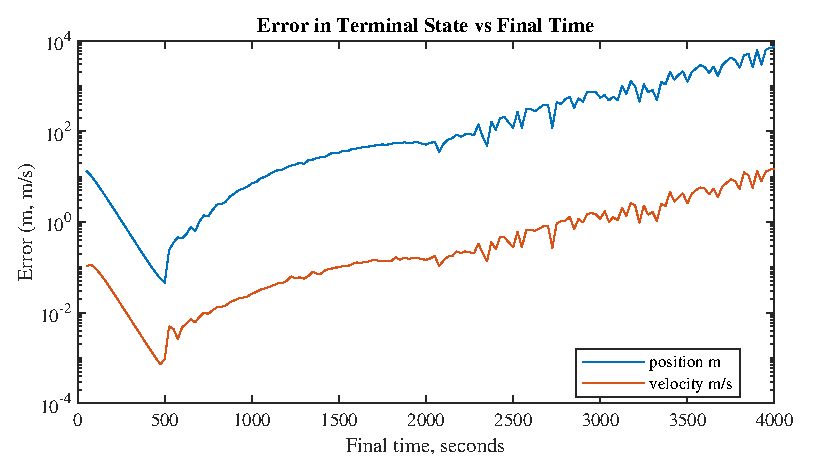
\includegraphics[width=0.5\textwidth]{figures/finaltime.eps}
  \caption{Hill Frame Position and Velocity Error vs Final Time}
  \label{fig:finaltime}
 \end{figure}
 It should also be understood that the larger the final time horizon, the more poorly conditioned the state transition matrix. The matrix may end up with entries that go below machine precision.
%
\subsection{Robustness Under Differing Conditions}
\subsubsection{Uncertain Initial State}
We shall now look at the performance of this controller with uncertainty in the initial condition $[r_0 \ v_0 \ \lambda_{r_0} \ \lambda_{v_0}]$. This implies that the initial $r, \ v$ and costate values are not correct, although are close to their real values; therefore, the control is not calculated correctly. For this case, we use an initial offset $r_0 + 0.5m, \ v_0 + 0.5 \frac{m}{s}$ to calculate the initial costate conditions. Note that the dynamics are integrated in kilometers, and therefore, this uncertain state is different by only $5\times10^{-4}$.
\begin{figure}[htpb!]
\begin{subfigure}{.5\textwidth}
  \centering
  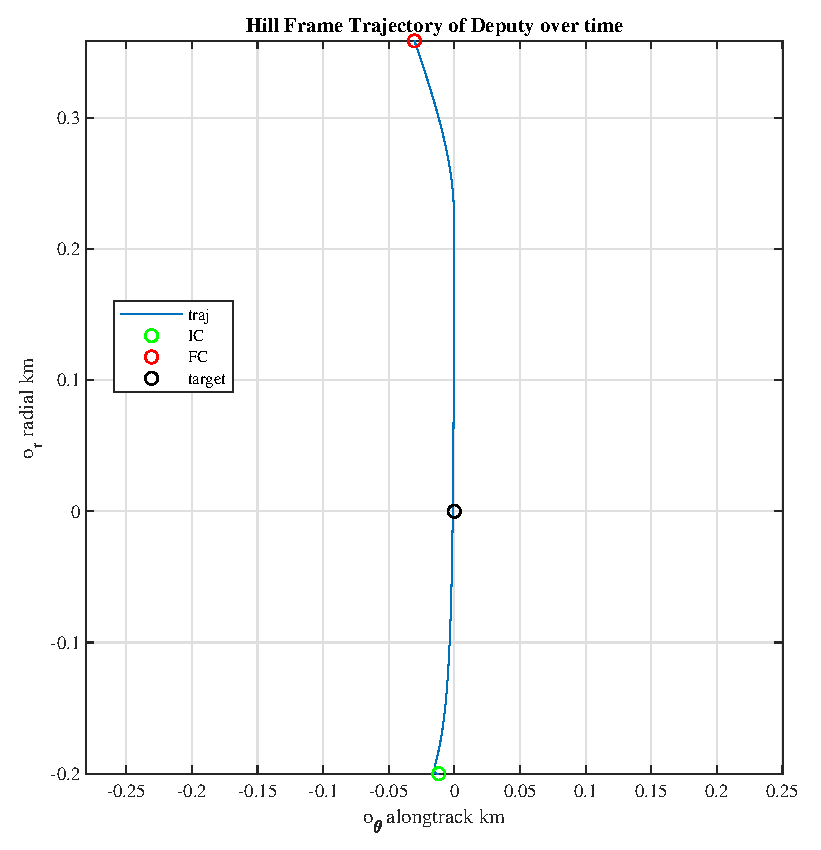
\includegraphics[width=.8\linewidth]{figures/traj_u.eps}
\end{subfigure}%
\begin{subfigure}{.5\textwidth}
  \centering
  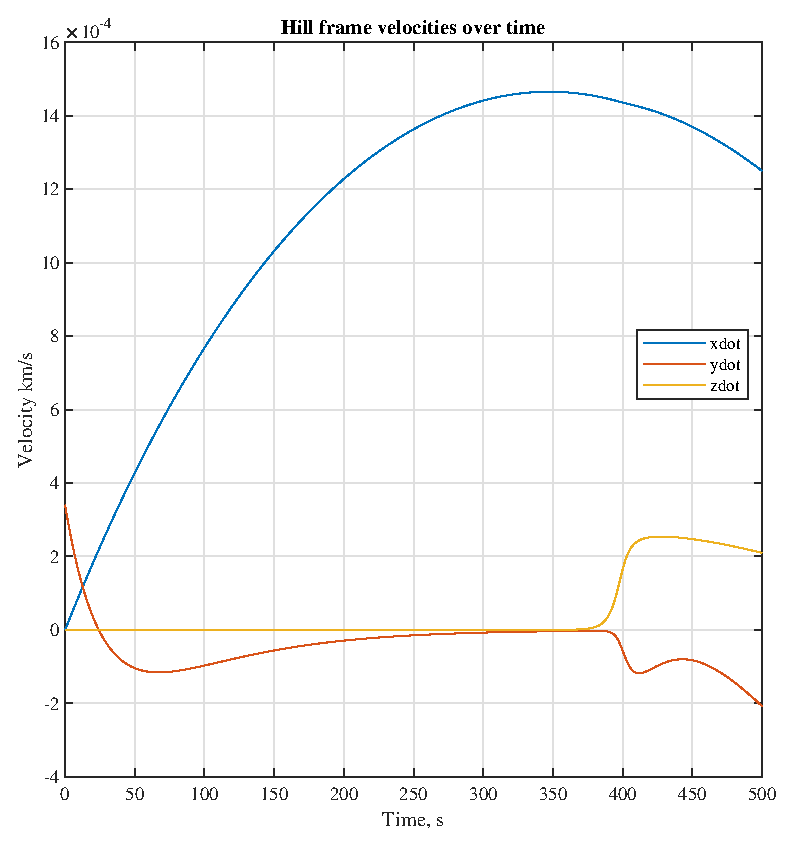
\includegraphics[width=.8\linewidth]{figures/vels_u.eps}
\end{subfigure}
\caption{Trajectory and Velocities Over Time}
\label{fig:uncertain}
\end{figure}

Clearly, the optimal with PD control overshoots the target wildly (over 300 meters), under very small initial condition uncertainty. This method seems to be highly sensitive to offsets, and performs badly. It may perform better if the algorithm is non-dimensionalized to get rid of numerical instabilities.


\subsubsection{Control Uncertainties}
Now, with deterministic initial condition values, let us look at what happens if the thruster input is stochastic. I modeled the thrust with additive white Gaussian noise of SNR 10 and looked at the response. This widened the terminal error to about $8.399$ meters in Hill frame displacement and $0.0488$ meters per second in Hill frame terminal velocity.

\begin{figure}[htpb!]
\begin{subfigure}{.5\textwidth}
  \centering
  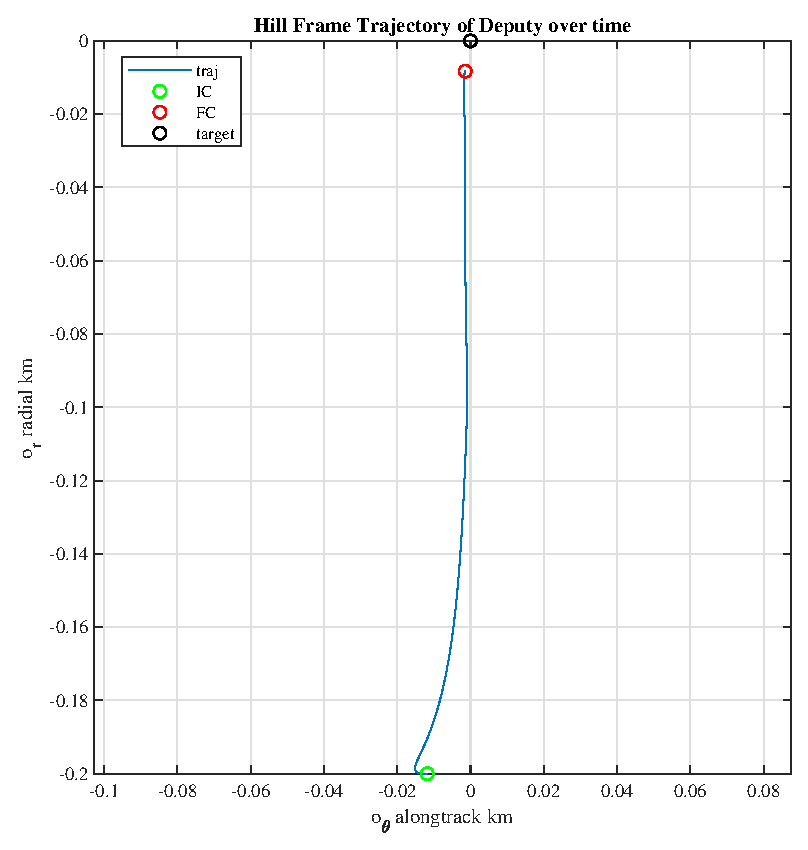
\includegraphics[width=.8\linewidth]{figures/traj_noise.eps}
\end{subfigure}%
\begin{subfigure}{.5\textwidth}
  \centering
  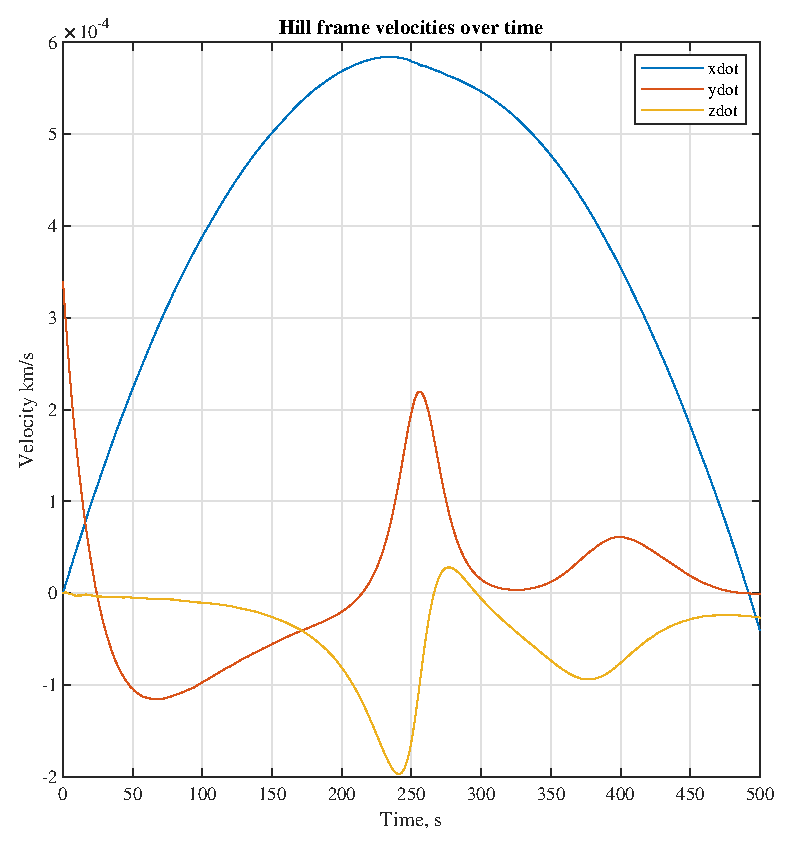
\includegraphics[width=.8\linewidth]{figures/vels_noise.eps}
\end{subfigure}
\caption{Trajectory and Velocities with Noisy Input Over Time}
\label{fig:noise}
\end{figure}
\begin{figure}[!htbp] 
  \centering
  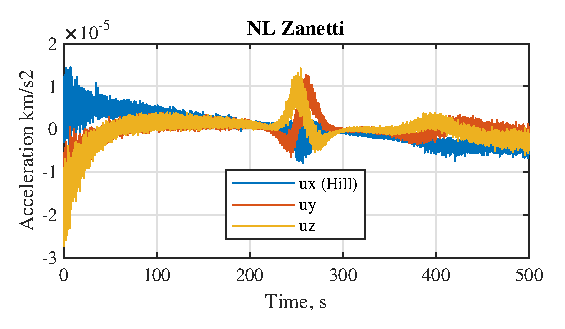
\includegraphics[width=0.5\textwidth]{figures/controls_noise.eps}
  \caption{Noisy Input Signal Over Time}
  \label{fig:unoise}
 \end{figure}


The system seems to behave better here than uncertainty in the initial condition. Performance may be improved by including an integral control term to zero out the steady state error incurred by stochastic thrust. This \textbf{completes Task 3}.


\section{Conclusion and Future Work}
Over all, the implementation and demonstration of this optimal control solution was educational experience. Because this tends to be sensitive to uncertainties in the initial condition as well as the final-time for implementation, I do not necessarily recommend using this solution. In the future, I would like to implement a closed loop safe rendezvous algorithm which allows many more constraints and can split up thrust to a matrix of different on-off gas thrusters.

\clearpage
\bibliographystyle{aiaa}   % Number the references.
\bibliography{references}   % Use references.bib to resolve the labels.




% \newpage
% \section*{Project Code}
% \lstinputlisting[caption = {Main Script (Simulation Framework)}]{../../project1_code/main.m}
% \lstinputlisting[caption = {Spacecraft Class}]{../../project1_code/spacecraft.m}
% \lstinputlisting[caption = {Nonlinear Relative ODEs}]{../../project1_code/nl_rel_ode.m}
% \lstinputlisting[caption = {CW ODEs}]{../../project1_code/cw_hill_ode.m}
% \lstinputlisting[caption = {Cart2Hill}]{../../project1_code/Cart2Hill.m}
% \lstinputlisting[caption = {RV2OE and OE2RV Utility}]{../../project1_code/schaub_elements.m}
% \lstinputlisting[caption = {Bounded Hill Orbit Test Script}]{../../project1_code/test_bounded.m}


\end{singlespace}
\end{document}